\section{Exploratory Data Analysis}

In this project, we work with the Heart Failure Prediction Dataset \cite{HeartFailurePrediction} on Kaggle, according to which ``Heart failure is a common event caused by CVDs and this dataset contains 11 features that can be used to predict a possible heart disease.''

The dataset contains $184$ rows of data. By inspection of the dataset columns, we split the features into numerical and categorical. The \textbf{numerical} features are:
\begin{itemize}
    \item \texttt{Age} -- all are integer values between 28 and 75, with no missing values, and a distribution close to normal.
    \item \texttt{RestingBP} -- integer values between 92--200, resembling a normal distribution. No missing values.
    \item \texttt{Cholesterol} -- integer values between 100--603, however, the column contains 31 missing values.
    \item \texttt{MaxHR} -- integer value between 71--202, close to normally distributed; no missing values.
    \item \texttt{Oldpeak} -- float values between $-2.6$--$4.0$. The distribution has more mass at the value $0.0$ suggesting that maybe some NaN values were formatted as $0.0$, but since there is no way for us to distinguish a NaN value from $0.0$, we decided to not process this further.
\end{itemize}
\begin{figure}[H]
    \centering
    \begin{subfigure}{0.19\columnwidth}
        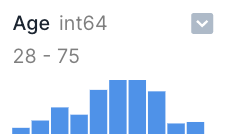
\includegraphics[width=1\textwidth]{images/feat_age.png}
    \end{subfigure}
    \begin{subfigure}{0.19\columnwidth}
        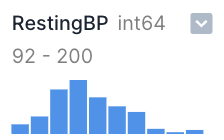
\includegraphics[width=1\textwidth]{images/feat_restingbp.png}
    \end{subfigure}
    \begin{subfigure}{0.19\columnwidth}
        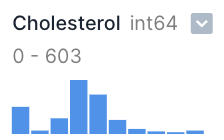
\includegraphics[width=1\textwidth]{images/feat_cholesterol.png}
    \end{subfigure}
    \begin{subfigure}{0.19\columnwidth}
        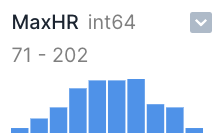
\includegraphics[width=1\textwidth]{images/feat_maxhr.png}
    \end{subfigure}
    \begin{subfigure}{0.19\columnwidth}
        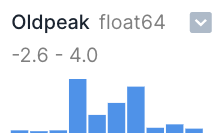
\includegraphics[width=1\textwidth]{images/feat_oldpeak.png}
    \end{subfigure}
    \caption{Visualized distributions of the numerical features.}
\end{figure}

The categorical features include:
\begin{enumerate}
    \item \texttt{Sex} -- admits values \texttt{M} ($82.6\%$, \texttt{F} with no missing values.
    \item \texttt{ChestPainType} -- admits values \texttt{ASY} (most common with $115$ instances), \texttt{NAP}, \texttt{ATA}, \texttt{TA}; no missing values.
    \item \texttt{FastingBS} -- admits values \texttt{0}, \texttt{1}. This feature is formatted as integers, so there is no need to transform it into a numerical value.
    \item \texttt{RestingECG} -- admits values \texttt{Normal} (most common), \texttt{LVH}, \texttt{ST}.
    \texttt{ExerciseAngina} -- a boolean feature with values \texttt{Y}, \texttt{N}.
    \item \texttt{ST\_Slope} -- has values \texttt{Flat} (most common), \texttt{Up}, \texttt{Down}.
\end{enumerate}
No categorical features have missing values.

Finally, the dataset has the column \texttt{HeartDisease} with values either \texttt{0} ($59.8\%$) and \texttt{1} ($40.2\%$), which is our target feature to predict. We observe that the classes are imbalanced. We account for that in the models described in the later sections by using the F1 score for evaluation.

\subsection{Data preprocessing}

For numerical features, we impute in missing values in the dataset using k-Nearest Neighbors (with $k=2$ and uniform weights).

Categorical features are encoded using one-hot encoding with one output feature for each class in the input. An exception are binary categorical features (namely \texttt{Sex} and \texttt{ExerciseAngina}) that are mapped only to a single binary numerical feature. Further, we decided to map values of the \texttt{ST\_Slope} feature by
\begin{align*}
\texttt{Up}\ &\mapsto\ 1\\
\texttt{Flat}\ &\mapsto\ 0\\
\texttt{Down}\ &\mapsto\ -1
\end{align*}
to allow models to make use of the ordinal relationship between the labels of this feature.
Using the described expands the 11 input features (mixed numerical and categorical) into 16 numerical features, see \autoref{fig:preprocessing_pipeline}.

\begin{figure}
    \centering
    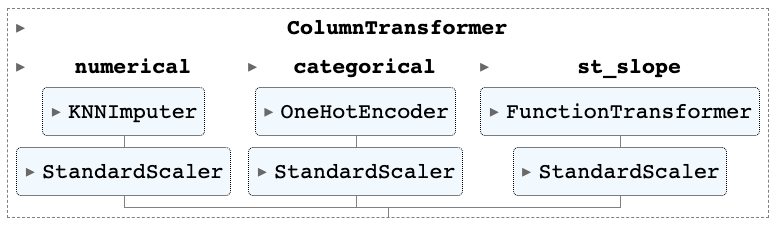
\includegraphics[width=1\columnwidth]{images/preprocessor_pipeline.png}
    \caption{Diagram showing the preprocessing pipeline}
    \label{fig:preprocessing_pipeline}
\end{figure}

Finally, we standardize the feature values by removing their mean and scaling them to unit variance.

\subsection{Train-Test Split}

We split the $184$ samples in the input dataset by $75\%/25\%$ randomly into a train dataset ($138$ samples) and a test dataset ($46$ samples). The operation, as well as all other random operations in the project, is deterministic and thus reproducible using a constant seed.

\subsection{First insights}

Figures \ref{fig:numerical_correlations} and \ref{fig:all_correlations} show correlation matrices between all features (including the target feature \texttt{HeartDisease}). From those, we observe that the most relevant features for heart disease prediction are: \texttt{ST\_Slope}, \texttt{ExerciseAngina}, \texttt{ChestPainType}, \texttt{MaxHR}. This suggests that models relying on these features for prediction will achieve a higher score.

\begin{figure}
    \centering
    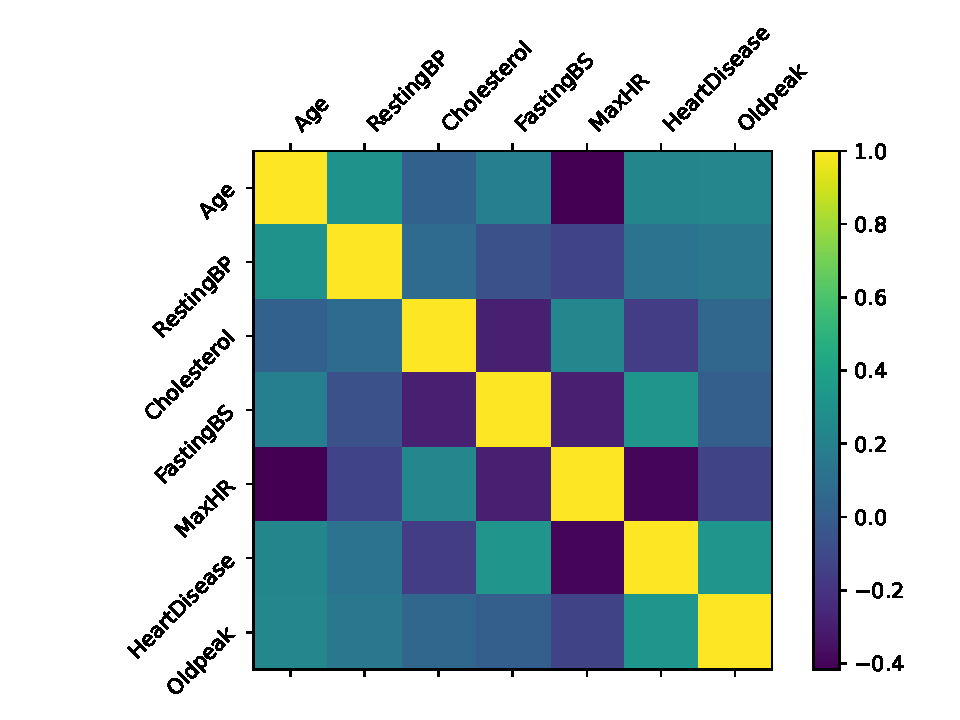
\includegraphics[width=1\columnwidth]{images/numerical_correlations.pdf}
    \caption{Correlation matrix of the numerical features}
    \label{fig:numerical_correlations}
\end{figure}
\begin{figure}
    \centering
    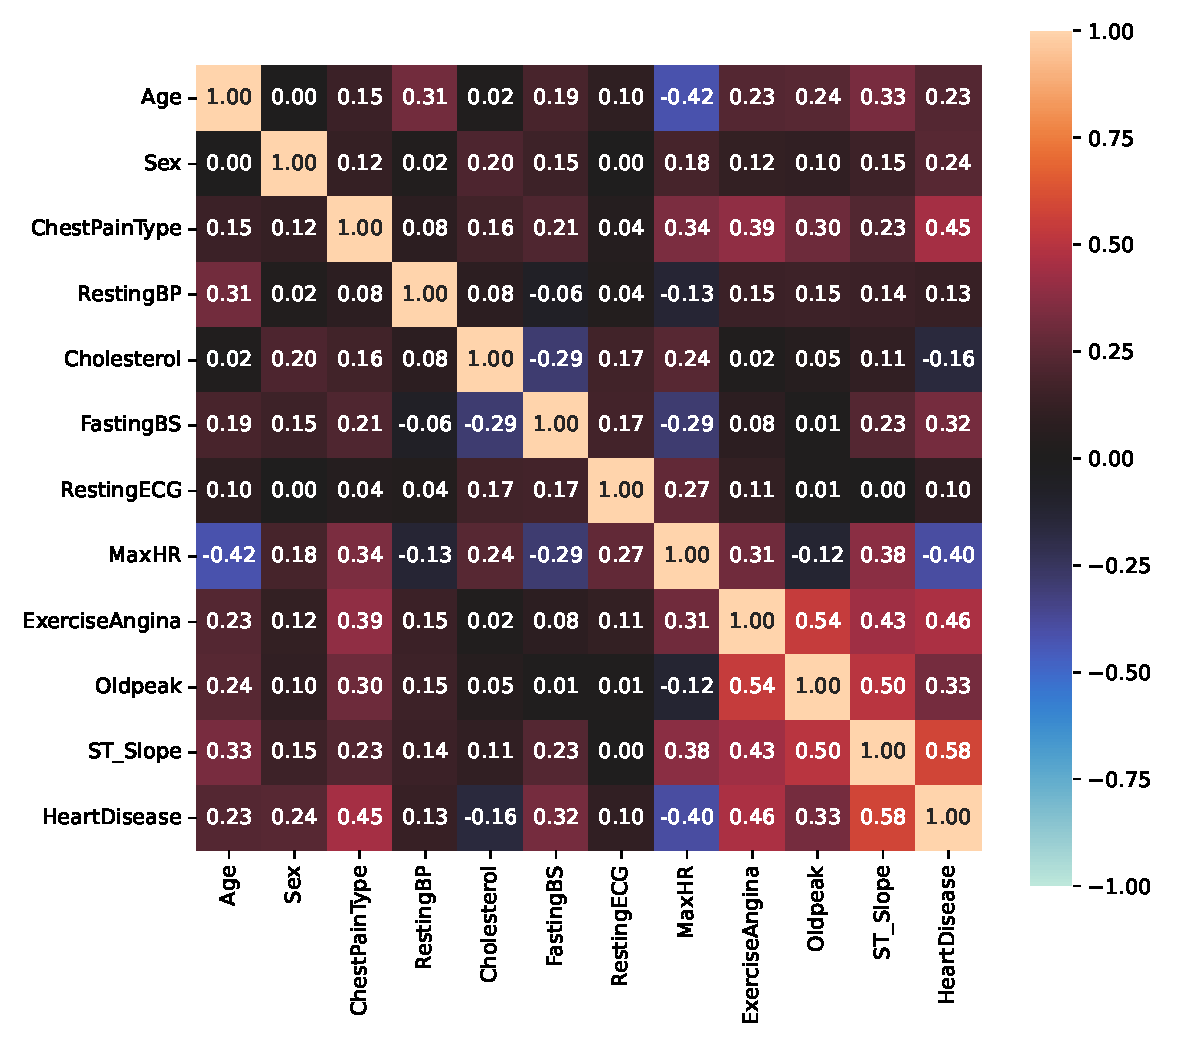
\includegraphics[width=1\columnwidth]{images/all_correlations.pdf}
    \caption{Convolution matrix of both numerical and categorical features using the \texttt{dython} Python library \cite{zychlinskiDython2023}, which uses ``Pearson's R for numerical-numerical cases, Correlation Ratio for categorical-numerical cases, and Cramer's V for categorical-categorical cases''.}
    \label{fig:all_correlations}
\end{figure}
\begin{figure*}
    \centering
    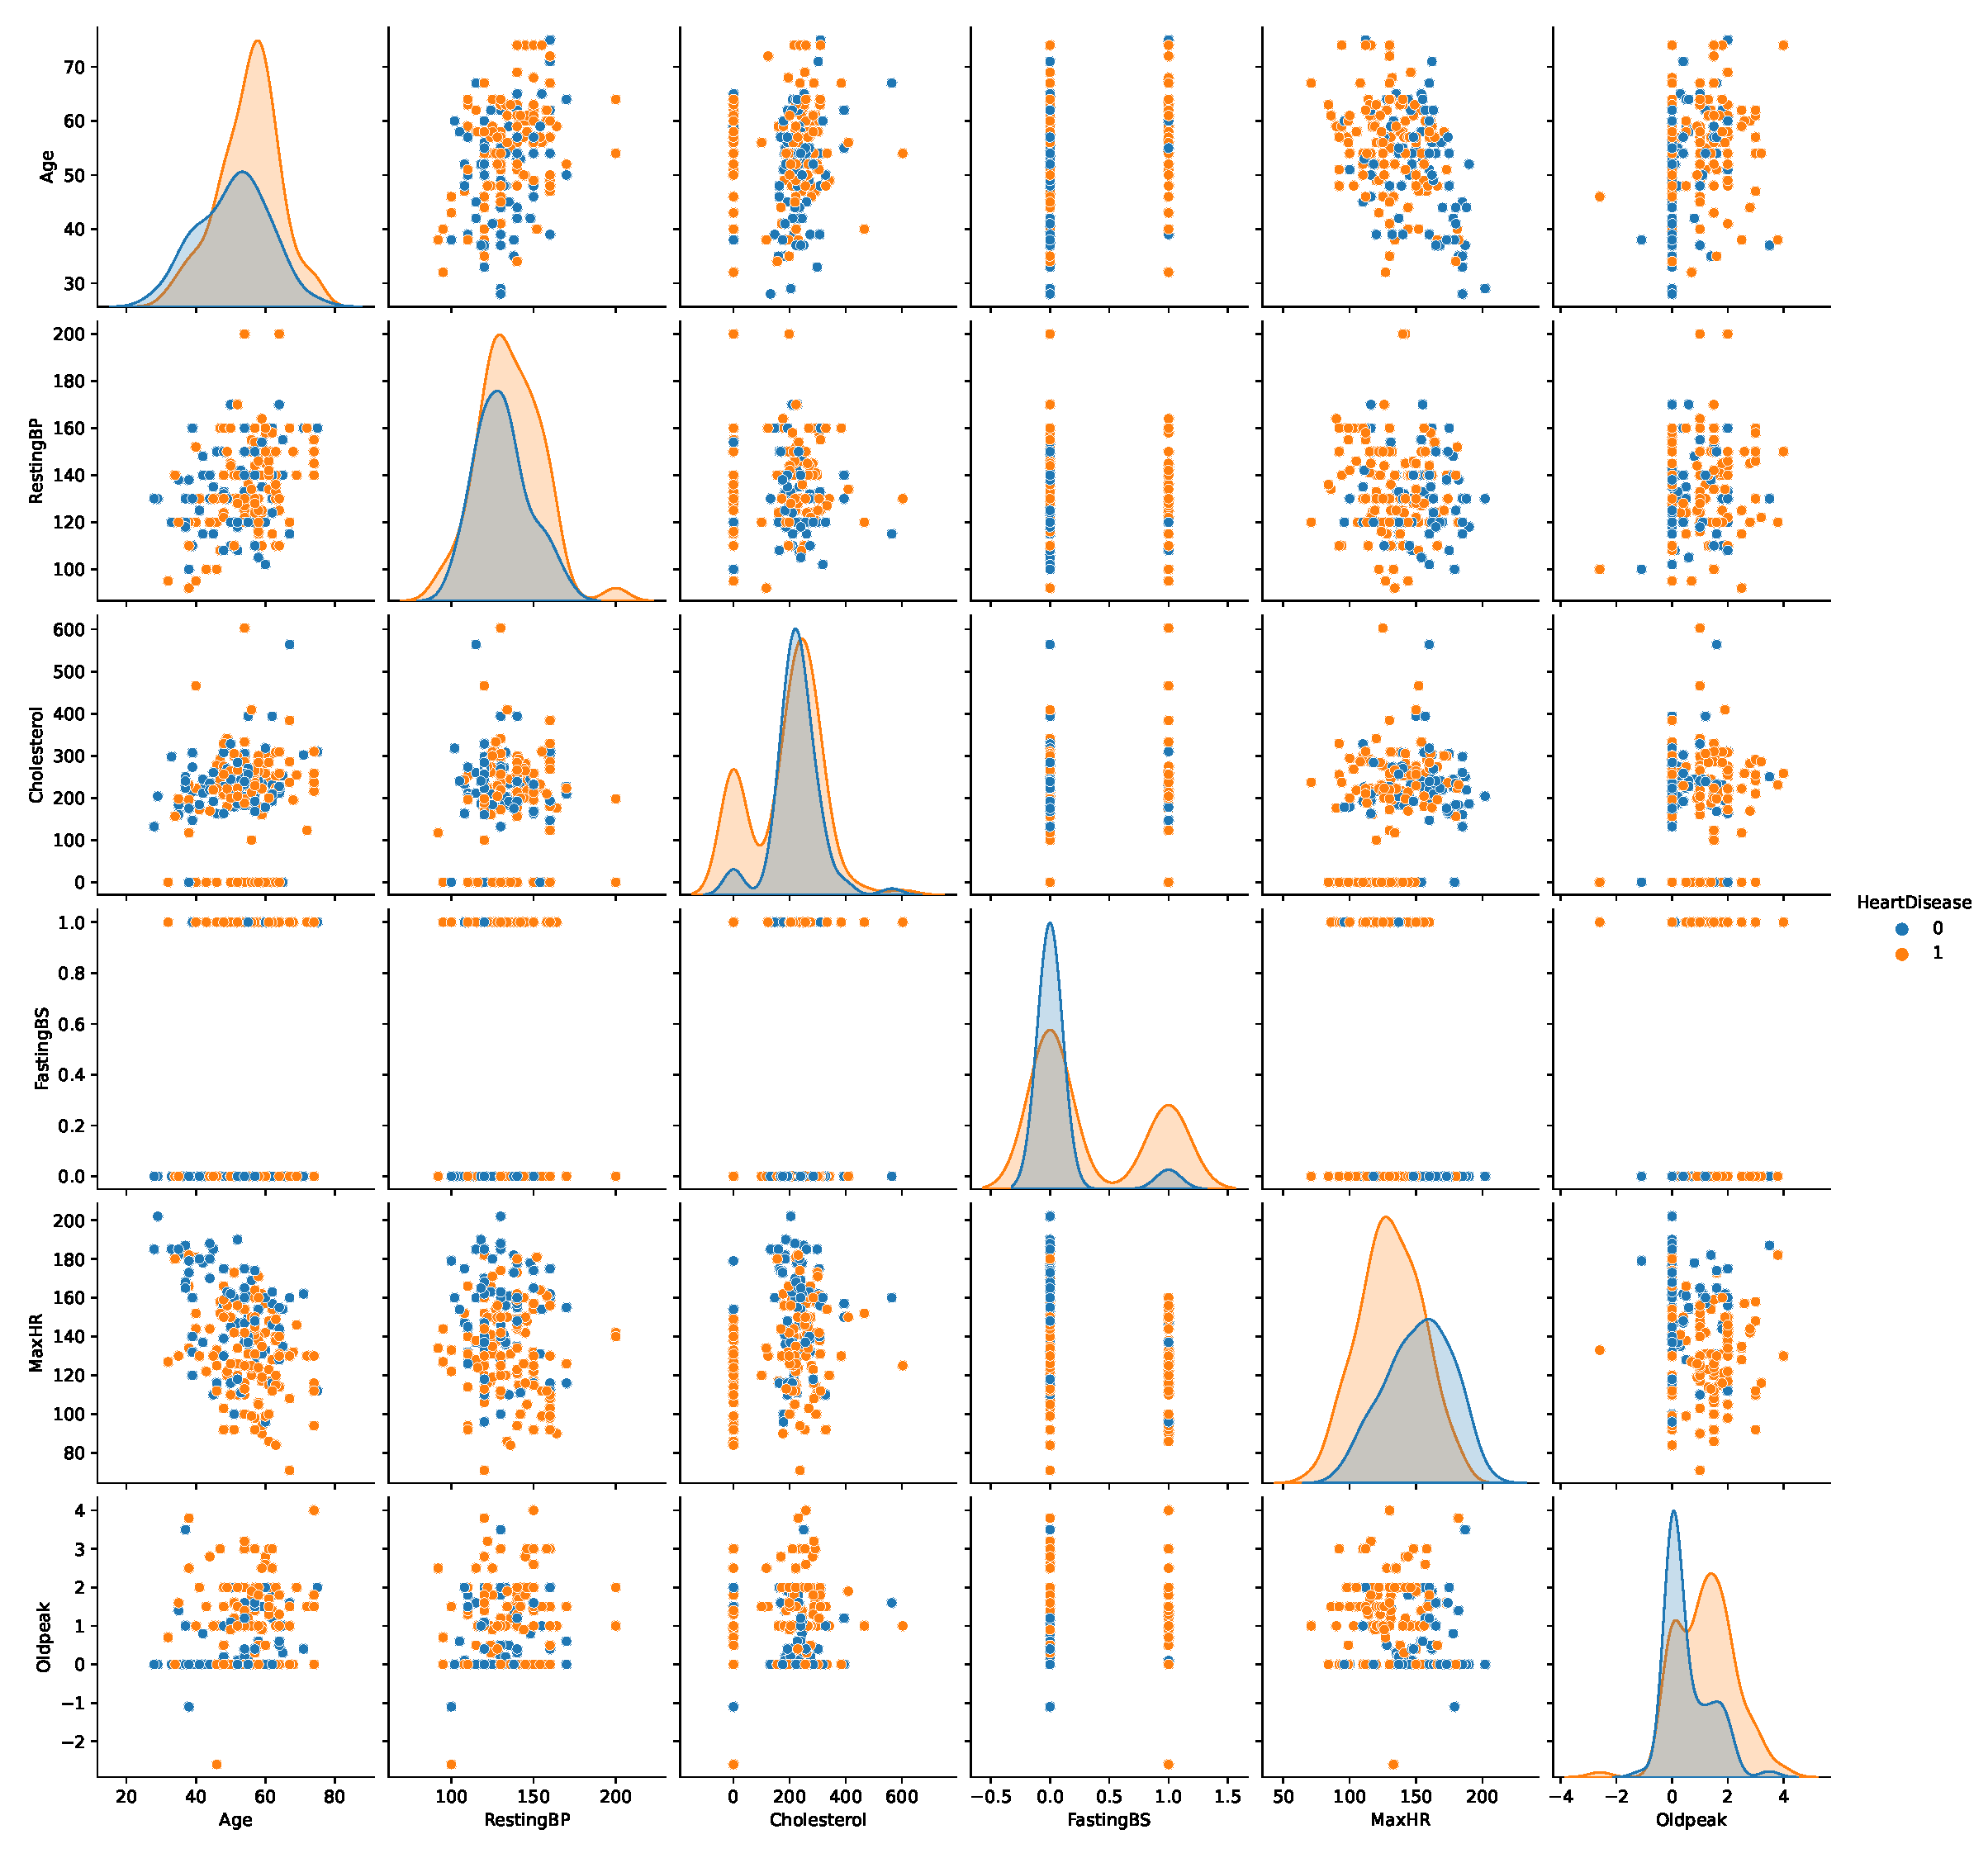
\includegraphics[width=1\textwidth]{images/pairplot.pdf}
    \caption{A plot showing pairwise relationships between numerical features in the dataset. Blue points represent samples without heart disease; orange points represent samples with heart disease.}
    \label{fig:pairplot}
\end{figure*}

\begin{figure}
    \centering
    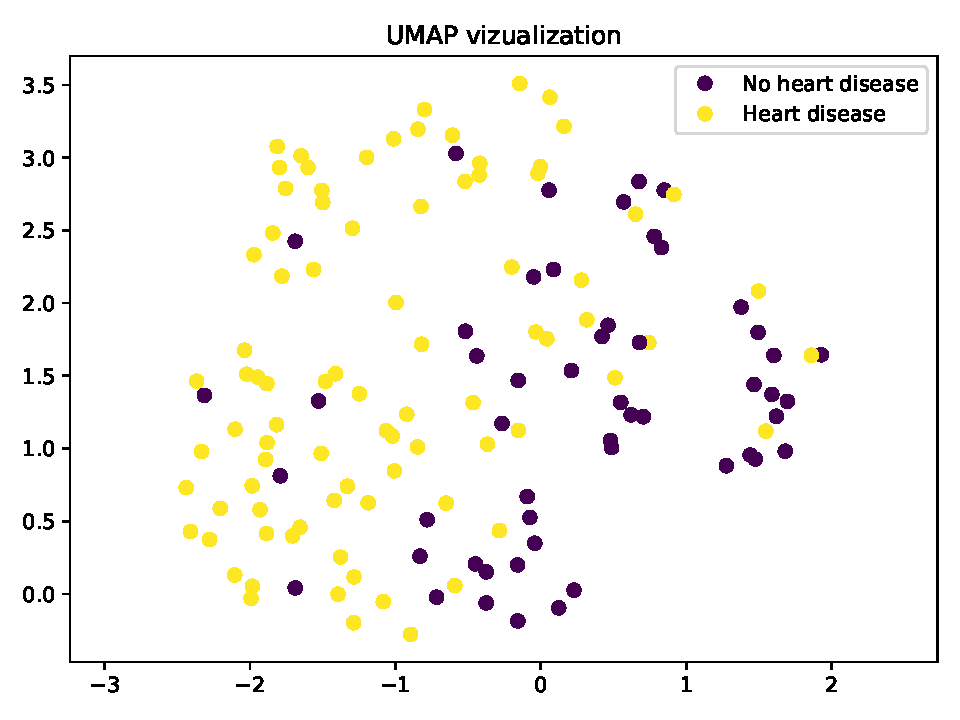
\includegraphics[width=1\columnwidth]{images/umap.pdf}
    \caption{The UMAP visualization \cite{mcinnesUMAPUniformManifold2020} of the training dataset in 2D.}
    \label{fig:umap}
\end{figure}

We also attach pairwise plots in \autoref{fig:pairplot}, which highlights the dependency of some features. As an example, the \texttt{Age}-\texttt{MaxHR} plot explains the negative correlation between the two features.

Additionally, in \autoref{fig:umap}, we analyze the training dataset visually using the UMAP dimensionality reduction tool \cite{mcinnesUMAPUniformManifold2020}. We observe that the dataset is at least to some extent linearly separable after the UMAP transformation even in two dimensions, which gives us an estimate of how well a good model should perform.
